\section{Accelerating Alice}\label{sec:acceleratingAlice}
	Recall how we performed the analysis in section \vref{sec:minkowskiAnalysis} using Minkowski spacetime diagrams.

	We used the fact that the relativistic Doppler effect causes both Alice and Donald to see the other person's clock running slowly when they are moving away from each other.
	We also used the fact that both Alice and Donald see the other person's clock running quickly when they are moving towards each other.

	Recall the formulas \eqref{eq:relDopAway} and \eqref{eq:relDopTowards} on page \pageref{eq:relDopAway}:
	\begin{samepagecols}{2}
		\paragraph{Moving away from each other}
		\begin{equation*}
			f_o = f_s \sqrt{\frac{1 - \beta}{1 + \beta}}
		\end{equation*}
		\paragraph{Moving towards each other}
		\begin{equation*}
			f_o = f_s \sqrt{\frac{1 + \beta}{1 - \beta}}
		\end{equation*}
	\end{samepagecols}
	\subsection{Magnitude of the Doppler effect}\label{subsec:dopMagnitude}
		Remember when we defined our notation in subsection \vref{subsec:notation} that $0 \leq \beta < 1$. Also, since division by 0 is not allowed, and a speed of 0 is not relevant, we will also place the restriction that $\beta \neq 0$, resulting in $0 < \beta < 1$.
		Next, we will analyze the magnitude of both formulas by simply graphing all $\beta$ values.
		See figure \ref{fig:dopplerAwayGraph} and \vref{fig:dopplerTowardsGraph}.
		\newpage
		\subsubsection{Moving away from each other}
			\begin{figure}[H]
	\caption{Graph of $f_o$ vs $\beta$ for the relativistic Doppler effect when Alice is moving away from Donald. Assuming $f_s = \SI{1}{\Hz}$, as it is in our example.}
	\label{fig:dopplerAwayGraph}
	\centering
	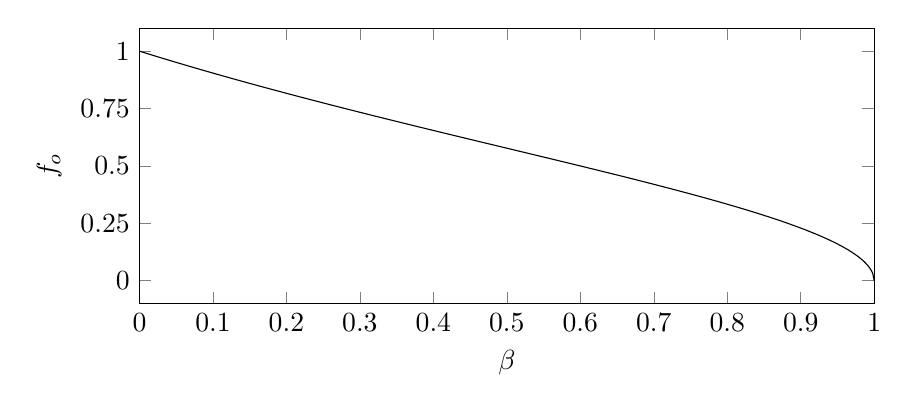
\begin{tikzpicture}
		\begin{axis}[
				xlabel=$\beta$,
				ylabel=$f_o$,
				xtick distance=0.1,
				ytick distance=0.25,
				width=0.9\textwidth,
				height=2in,
				xmin=0,
				xmax=1,
			]
			\addplot[
				domain=0:1,
				samples=501,
			]
			{sqrt((1-x)/(1+x))};
		\end{axis}
	\end{tikzpicture}
\end{figure}

			From this graph, we can see that both Alice and Donald will always see each other's clocks running slowly when they are moving away from each other.
		\subsubsection{Moving towards each other}
			\begin{figure}[H]
	\caption{Graph of $f_o$ vs $\beta$ for the relativistic Doppler effect when Alice is moving towards Donald. Assuming $f_s = \SI{1}{\Hz}$, as it is in our example.}
	\label{fig:dopplerTowardsGraph}
	\centering
	\begin{tikzpicture}
		\begin{axis}[
				xlabel=$\beta$,
				ylabel=$f_o$,
				xtick distance=0.1,
				ytick distance=1,
				width=0.9\textwidth,
				height=2in,
				xmin=0,
				xmax=1,
				ymin=0,
				ymax=5,
			]
			\addplot[
				domain=0:1,
				samples=501,
			]
			{sqrt((1+x)/(1-x))};
		\end{axis}
	\end{tikzpicture}
\end{figure}

			From this graph, we can see that both Alice and Donald will always see each other's clocks running quickly when they are moving towards each other. This graph goes to infinity in the portion that was cutoff because it could not fit on the page.
	\subsection{Implications of subsection \ref{subsec:dopMagnitude}}
		From \ref{fig:dopplerAwayGraph} and \vref{fig:dopplerTowardsGraph} we see that no matter the value of $\beta$, Alice and Donald will observe time speed up and slow down in the same way as in our example with an inertial frame of reference, just by different amounts.
		However, as they move away from each other, they will both always see a slow clock for the other person.
		And as they move towards each other, they will both always see a fast clock for the other person.

		Remember that while doing our calculations, what mattered to get the results we did was that both Alice and Donald saw the other person's clock running slowly on the outbound leg, and quickly on the inbound leg. A different value of $\beta$ would change how much dilation occurs, but would not change the fact that dilation is occurring.

		We can draw out the world lines for what would happen if Alice was accelerating. See figure \vref{fig:acceleratingClassicalMinkowski} to help with visualization, and figures \ref{fig:acceleratingDonaldMinkowski} and \vref{fig:acceleratingAliceInDonaldMinkowski} for what actually happens.
		\begin{figure}[H]
	\begin{minipage}{0.3\textwidth}
		\caption{Minkowski spacetime diagram of what we would expect to see according to classical physics with Donald as the frame of reference, if Alice accelerates to speed up, turn around, and stop.}
		\label{fig:acceleratingClassicalMinkowski}
	\end{minipage}
	\hfill
	\begin{minipage}{0.6\textwidth}
		\begin{tikzpicture}
			\begin{axis}[
					xlabel=$d\ (\si{\lightyear})$,
					ylabel=$t\ (\si{\year})$,
					xmin=0,
					xmax=4.25,
					ymin=0,
					ymax=10.75,
					xtick distance=1,
					ytick distance=1,
					height=4in,
					width=4in,
				]
				\addplot+[smooth] plot coordinates {
				(0,0)
				(4,5)
				(0,10)
				};
			\end{axis}
		\end{tikzpicture}
	\end{minipage}
\end{figure}

		\begin{figure}[H]
	\begin{minipage}{0.25\textwidth}
		\caption{Minkowski spacetime diagram of what Donald will see on his own clock, if Alice is accelerating for her whole journey.}
		\label{fig:acceleratingDonaldMinkowski}
	\end{minipage}
	\hfill
	\begin{minipage}{0.7\textwidth}
		\begin{tikzpicture}
			\begin{axis}[
					xlabel=$d\ (\si{\lightyear})$,
					ylabel=$t\ (\si{\year})$,
					xmin=0,
					xmax=4.25,
					ymin=0,
					ymax=10.75,
					xtick distance=1,
					ytick distance=1,
					height=3.5in,
					width=4in,
				]
				\addplot+[smooth] plot coordinates {
				(0,0)
				(4,9)
				(0,10)
				};
			\end{axis}
		\end{tikzpicture}
	\end{minipage}
\end{figure}

		\begin{figure}[H]
	\begin{minipage}{0.25\textwidth}
		\caption{Minkowski spacetime diagram of what Alice will see in Donald's clock, if Alice accelerates to speed up, turn around, and stop.}
		\label{fig:acceleratingAliceInDonaldMinkowski}
	\end{minipage}
	\hfill
	\begin{minipage}{0.7\textwidth}
		\begin{tikzpicture}
			\begin{axis}[
					xlabel=$d\ (\si{\lightyear})$,
					ylabel=$t\ (\si{\year})$,
					xmin=0,
					xmax=4.25,
					ymin=0,
					ymax=10.75,
					xtick distance=1,
					ytick distance=1,
					height=3.5in,
					width=4in,
				]
				\addplot+[smooth] plot coordinates {
				(0,0)
				(4,1)
				(0,10)
				};
			\end{axis}
		\end{tikzpicture}
	\end{minipage}
\end{figure}

		\newpage
		Now that we have the different world lines, we need to figure out what changes in our calculations.

		In our calculations in section \vref{sec:minkowskiAnalysis}, we used the distance from earth to the turnaround, the time it takes to get there, and the effects of the relativistic Doppler effect. Velocity was only used to calculate the relativistic Doppler effect, and to calculate how long the trip takes.

	\subsection{Conclusion of the accelerating twin paradox resolution}
		In our new world lines, we kept the distance and time the same.
		We also showed before that the Doppler effect will act in the same direction, but with a different magnitude as velocity changes.
		The only other thing that has changed at any point of the world lines is velocity, since acceleration is simply the derivative of velocity.
		But, again, velocity was only used to initially calculate the length of the trip.
		Leaving the length of the trip the same, and varying velocity over time (applying acceleration), we see that nothing will change our solution to the paradox. All that will change is the amount of time dilation\footnote{Doing the actual calculations for this is quite complicated. In the second half of this paper, we will approach these calculation with a computer simulation.}, but the paradox remains solved.

		Finally, we can consider the twin paradox to be completely resolved for both infinite and finite accelerations.
